%%% neutron.tex --- 

%% Author: Antonio Messina
%% Version: $Id: neutron.tex,v 0.0 2014/08/30 08:34:18 antonio Exp$

%%\revision$Header: /home/antonio/git/gridka-school/presentations/neutron/neutron.tex,v 0.0 2014/08/30 08:34:18 antonio Exp$

\documentclass[english,serif,mathserif,xcolor=pdftex,dvipsnames,table]{beamer}
\usetheme[formal]{s3it}
\usepackage{s3it}

\author{%
  {\bfseries Antonio Messina \texttt{<antonio.messina@s3it.uzh.ch>}}  
}

\institute[UZH]{%
  S$^3$IT - Services and Support for Science IT,
  University of Zurich
}

\title[Neutron]{OpenStack networking\\Neutron}
\date{4~September~2014}

\setbeamertemplate{itemize
  item}{\color{uzh@blue}\scriptsize\raise1.25pt\hbox{$\bullet$}}

\begin{document}
\begin{frame}
  \titlepage
\end{frame}

\begin{frame}[fragile]
  \frametitle{Why neutron?}
  \begin{itemize}
  \item Allow tenants to define the network topology
  \item Support very rich network topologies.
    \begin{itemize}
    \item including existing topologies
    \end{itemize}
  \item Allow easy integration with network infrastructure.
  \item Allow creation of advanced network services, like:
    \begin{itemize}
    \item load balancing
    \item VPN
    \item firewall
    \end{itemize}
  \end{itemize}

  \+
  {\footnotesize\url{https://wiki.openstack.org/wiki/Neutron}}

\end{frame}


\begin{frame}
  {main building blocks}
% from http://ilearnstack.com/2013/10/07/networking-in-openstack-panoramic-view/
  \begin{figure}
    \centering
    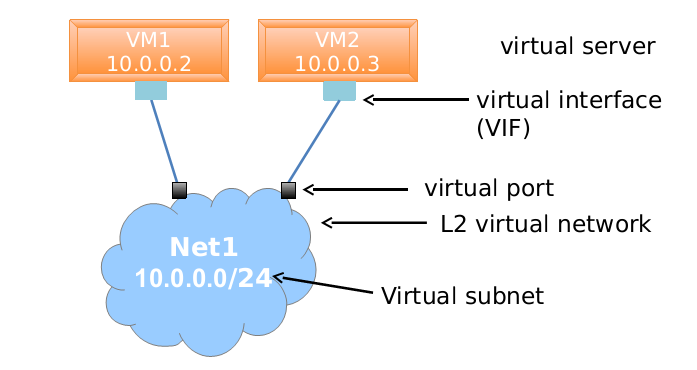
\includegraphics[width=0.9\linewidth]{neutron_concept}
  \end{figure}
\begin{description}
\item[network] A L2 network
\item[subnet] An IPv4 or IPv6 network, living inside a \texttt{network}
\item[port] a virtual switch port on a given \texttt{network}.
\item[virt. interface] instance interface, connected to a \texttt{port}
\end{description}
\end{frame}

\begin{frame}
  {Neutron architecture}
  \begin{description}
  \item[neutron server] rest API, talks to DB and AMQP
  \item[plugin agent] runs on each compute node, manage virtual
    switches and ports
  \item[DHCP agent] provides DHCP services to tenant networks
  \item[L3 agent] provides routing and NAT capabilities
  \item[SDN services] additional network services
  \end{description}
\end{frame}


% neutron server (neutron-server and neutron-*-plugin)
%
%     This service runs on the network node to service the Networking API
%     and its extensions. It also enforces the network model and IP
%     addressing of each port. The neutron-server and plugin agents require
%     access to a database for persistent storage and access to a message
%     queue for inter-communication.  
%
% plugin agent (neutron-*-agent)
%
%     Runs on each compute node to manage local virtual switch (vswitch)
%     configuration. The plug-in that you use determine which agents
%     run. This service requires message queue access. Optional depending on
%     plugin.  
%
% DHCP agent (neutron-dhcp-agent)
%
%     Provides DHCP services to tenant networks. This agent is the same
%     across all plug-ins and is responsible for maintaining DHCP
%     configuration. The neutron-dhcp-agent requires message queue access.
%
% L3 agent (neutron-l3-agent)
%
%     Provides L3/NAT forwarding for external network access of VMs on
%     tenant networks. Requires message queue access. Optional depending on
%     plug-in.  
%
% network provider services (SDN server/services)
%
%     Provide additional networking services to tenant networks. These SDN
%     services might interact with the neutron-server, neutron-plugin,
%     and/or plugin-agents through REST APIs or other communication
%     channels.

\begin{frame}{Neutron services integrations}
  Neutron server, plugins and agents talk to each other via:
  \begin{itemize}
  \item rest API
  \item RPC (RabbitMQ in our case)
  \item SQL (MySQL in our case)
  \end{itemize}
  \begin{figure}
    \centering
    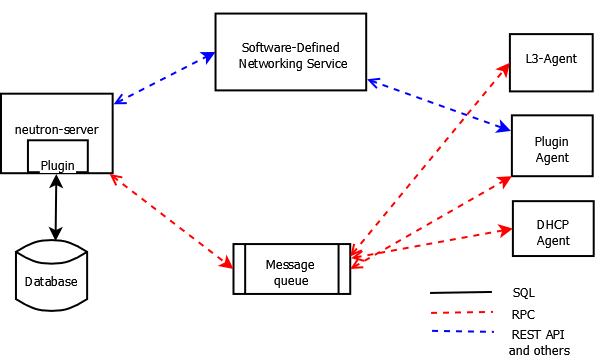
\includegraphics[width=0.8\linewidth]{sdn-connections}
  \end{figure}
  % neutron-server talks to -> database + message queue
  % message queue talks to -> L2 agent (to wire ports) (one for each
  % hypervisor usually)
  % and the dhcp agent (one per network)
  % and L3 agent (possibly one per network)
  % and to advanced agents (lbaas, fwaas, vpnaas)
\end{frame}

\begin{frame}
  {Neutron architecture - physical servers}

  \begin{figure}
    \centering    
    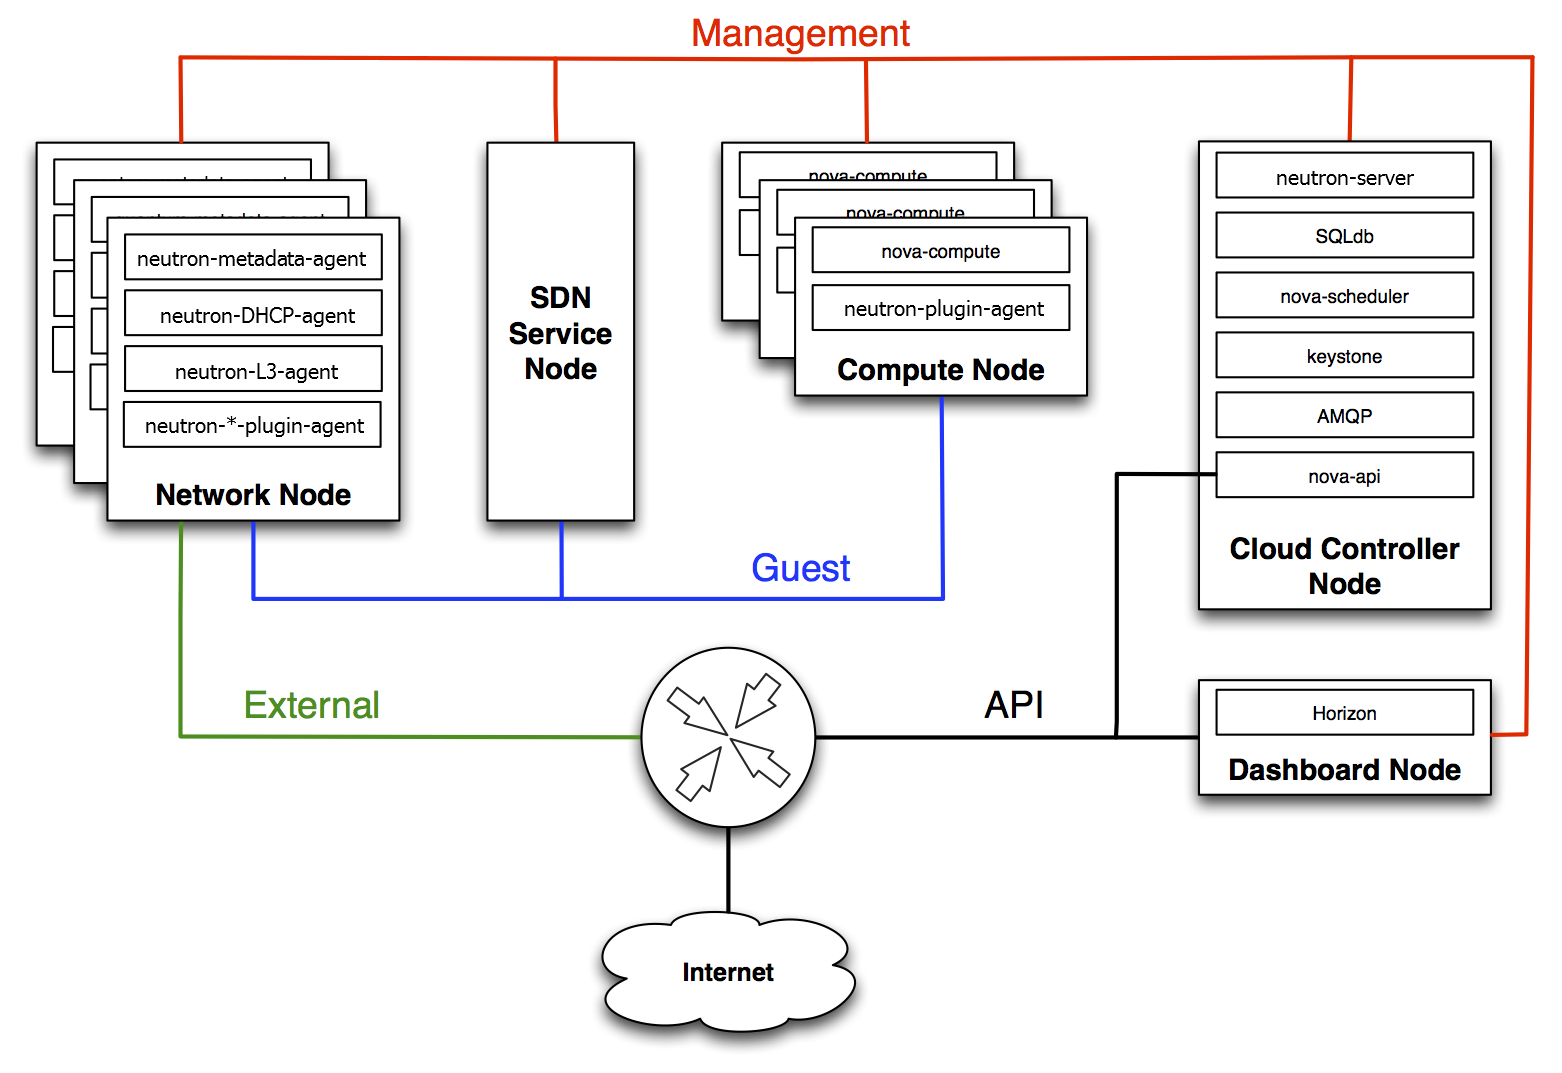
\includegraphics[width=0.9\linewidth]{1aa-network-domains-diagram}
  \end{figure}

  \begin{itemize}
  \item In our case, the \textbf{Network Node} is \textbf{neutron-node}
  \item We will install \texttt{neutron-server} on \textbf{neutron-node}
  \end{itemize}
\end{frame}

% \begin{frame}
%   {neutron server}
%   three parts:
%   \begin{itemize}
%   \item rest api (WSGI python app, listening to port 9696)
%   \item rpc service (AMQP)
%   \item plugin
%     \begin{itemize}
%     \item written in python
%     \item only one is active (option \texttt{core\_plugin} in \texttt{neutron.conf})
%     \item talk using API
%     \item optional db access
%     \item optional extensions
%     \end{itemize}
%   \end{itemize}
% \end{frame}

% \begin{frame}
%   {Plugin extensions}
%   are automatically discovered, and includes:
%   \begin{itemize}
%   \item binding
%   \item dhcp
%   \item L3
%   \item quota
%   \item security groups
%   \item extra routes
%   \item metering
%   \end{itemize}
% \end{frame}

\begin{frame}
  {ML2 plugin (since Havana/Icehouse)}
  \begin{itemize}
  \item Only one plugin is active in neutron at a time.
  \item ML2 plugin allow to use multiple L2 networking technologies at the
    same time.
  \item Being modular, reduce duplication of code, and makes easier create
    plugins for Neutron.

  \item Decouple the \textit{type} of network and its \textit{implementation}:
    \begin{description}
    \item[type driver] (GRE, VLAN, VXLAN, Flat)
    \item[mechanism driver] specific implementation for a specific
      network technology (OpenVSwitch, cisco, brocade \ldots)
    \end{description}
  \end{itemize}
\+
{\footnotesize\url{https://wiki.openstack.org/wiki/Neutron/ML2}}
\end{frame}

\begin{frame}
  {L2 agent}
  \begin{itemize}
  \item usually runs on the hypervisor
  \item talks to server via RPC
  \item watch and notify when devices are added/removed
  \item wires new devices ensuring:
    \begin{itemize}
    \item they are in the proper network segment (L2 network)
    \item security group rules are applied
    \end{itemize}
  \end{itemize}

  \+
  We will deploy \texttt{neutron-openvswitch-agent}

  \+
  {\footnotesize\url{http://openvswitch.org/}}
\end{frame}

% \begin{frame}
%   {The OVS L2 agent}
% Isolation is performed using VLAN, or GRE tunnels (or VXLAN)

% \end{frame}

\begin{frame}[fragile]
  \frametitle{Linux Network Namespaces}
A namespace is an \textit{isolated copy} of the network stack

\begin{itemize}
\item Each namespace has its own private loopback.
\item Routing is local to the namespace.
\item Addressing scope limited to the namespace
  \begin{itemize}
  \item[$\Rightarrow$] different namespaces can have overlapping IP addresses
  \end{itemize}
\item Interfaces \textbf{do not have} direct connectivity to the
  network: you must connect them to a bridge in the default namespace
\item You can spawn processes within a namespace
  (e.g. \texttt{dnsmasq} for DHCP)
\end{itemize}

\footnotesize
\begin{verbatim}
ip netns help
\end{verbatim}
{\footnotesize\href{http://lwn.net/Articles/531114/}{LWN.net: Namespaces
    in operation}}
\end{frame}


\begin{frame}
  {DHCP configuration agent}
  \begin{itemize}
  \item RPC based notifications
  \item uses \texttt{dnsmasq} (one per network)
  \item uses namespaces (\texttt{qdhcp-<uuid-of-neutron-subnet>})
  \item typically runs on the network node
  \item tap interface \texttt{tap-XXX} with \textit{private IP}, wired
    to \texttt{br-int}
  \item you can have multiple copies to achieve HA (part of DHCP:
    multiple servers cun run on the same network segment, the client
    gets the first response)\footnote{as long as the conf is the same}
  \end{itemize}
\end{frame}

\begin{frame}
  {L3 agent}

  Responsible for routing and floating IPs.

\scriptsize  \begin{itemize}
  \item Runs on the network node (typically).

  \item Uses namespaces (\texttt{qrouter-<uuid-of-neutron-router>})

  \item Also provides metadata agent.

  \item Routing is done with static routes.
    \begin{itemize}\scriptsize
    \item[$\Rightarrow$] linux forwarding must be enabled
    \end{itemize}
  \item tap interface \texttt{qg-X} with \textit{public} IP, wired to
    \texttt{br-ex} external bridge

  \item tap interface \texttt{qr-X} with \textit{private} IP, wired to
    \texttt{br-int}.

  \item IP on \texttt{qr-X} is the gateway for the tenant network.

  \item When using floating IPs, the L3 agent will assign the floating
    ip to \texttt{qg-X} and set in place a 1:1 NAT between public and
    private IPs.

  \item Otherwise, the L3 agent simply use NAT (MASQUERADE) to allow
    external connectivity (using the IP of \texttt{qg-X} interface)
  \end{itemize}
\end{frame}

\begin{frame}{Under the hood - network node}
  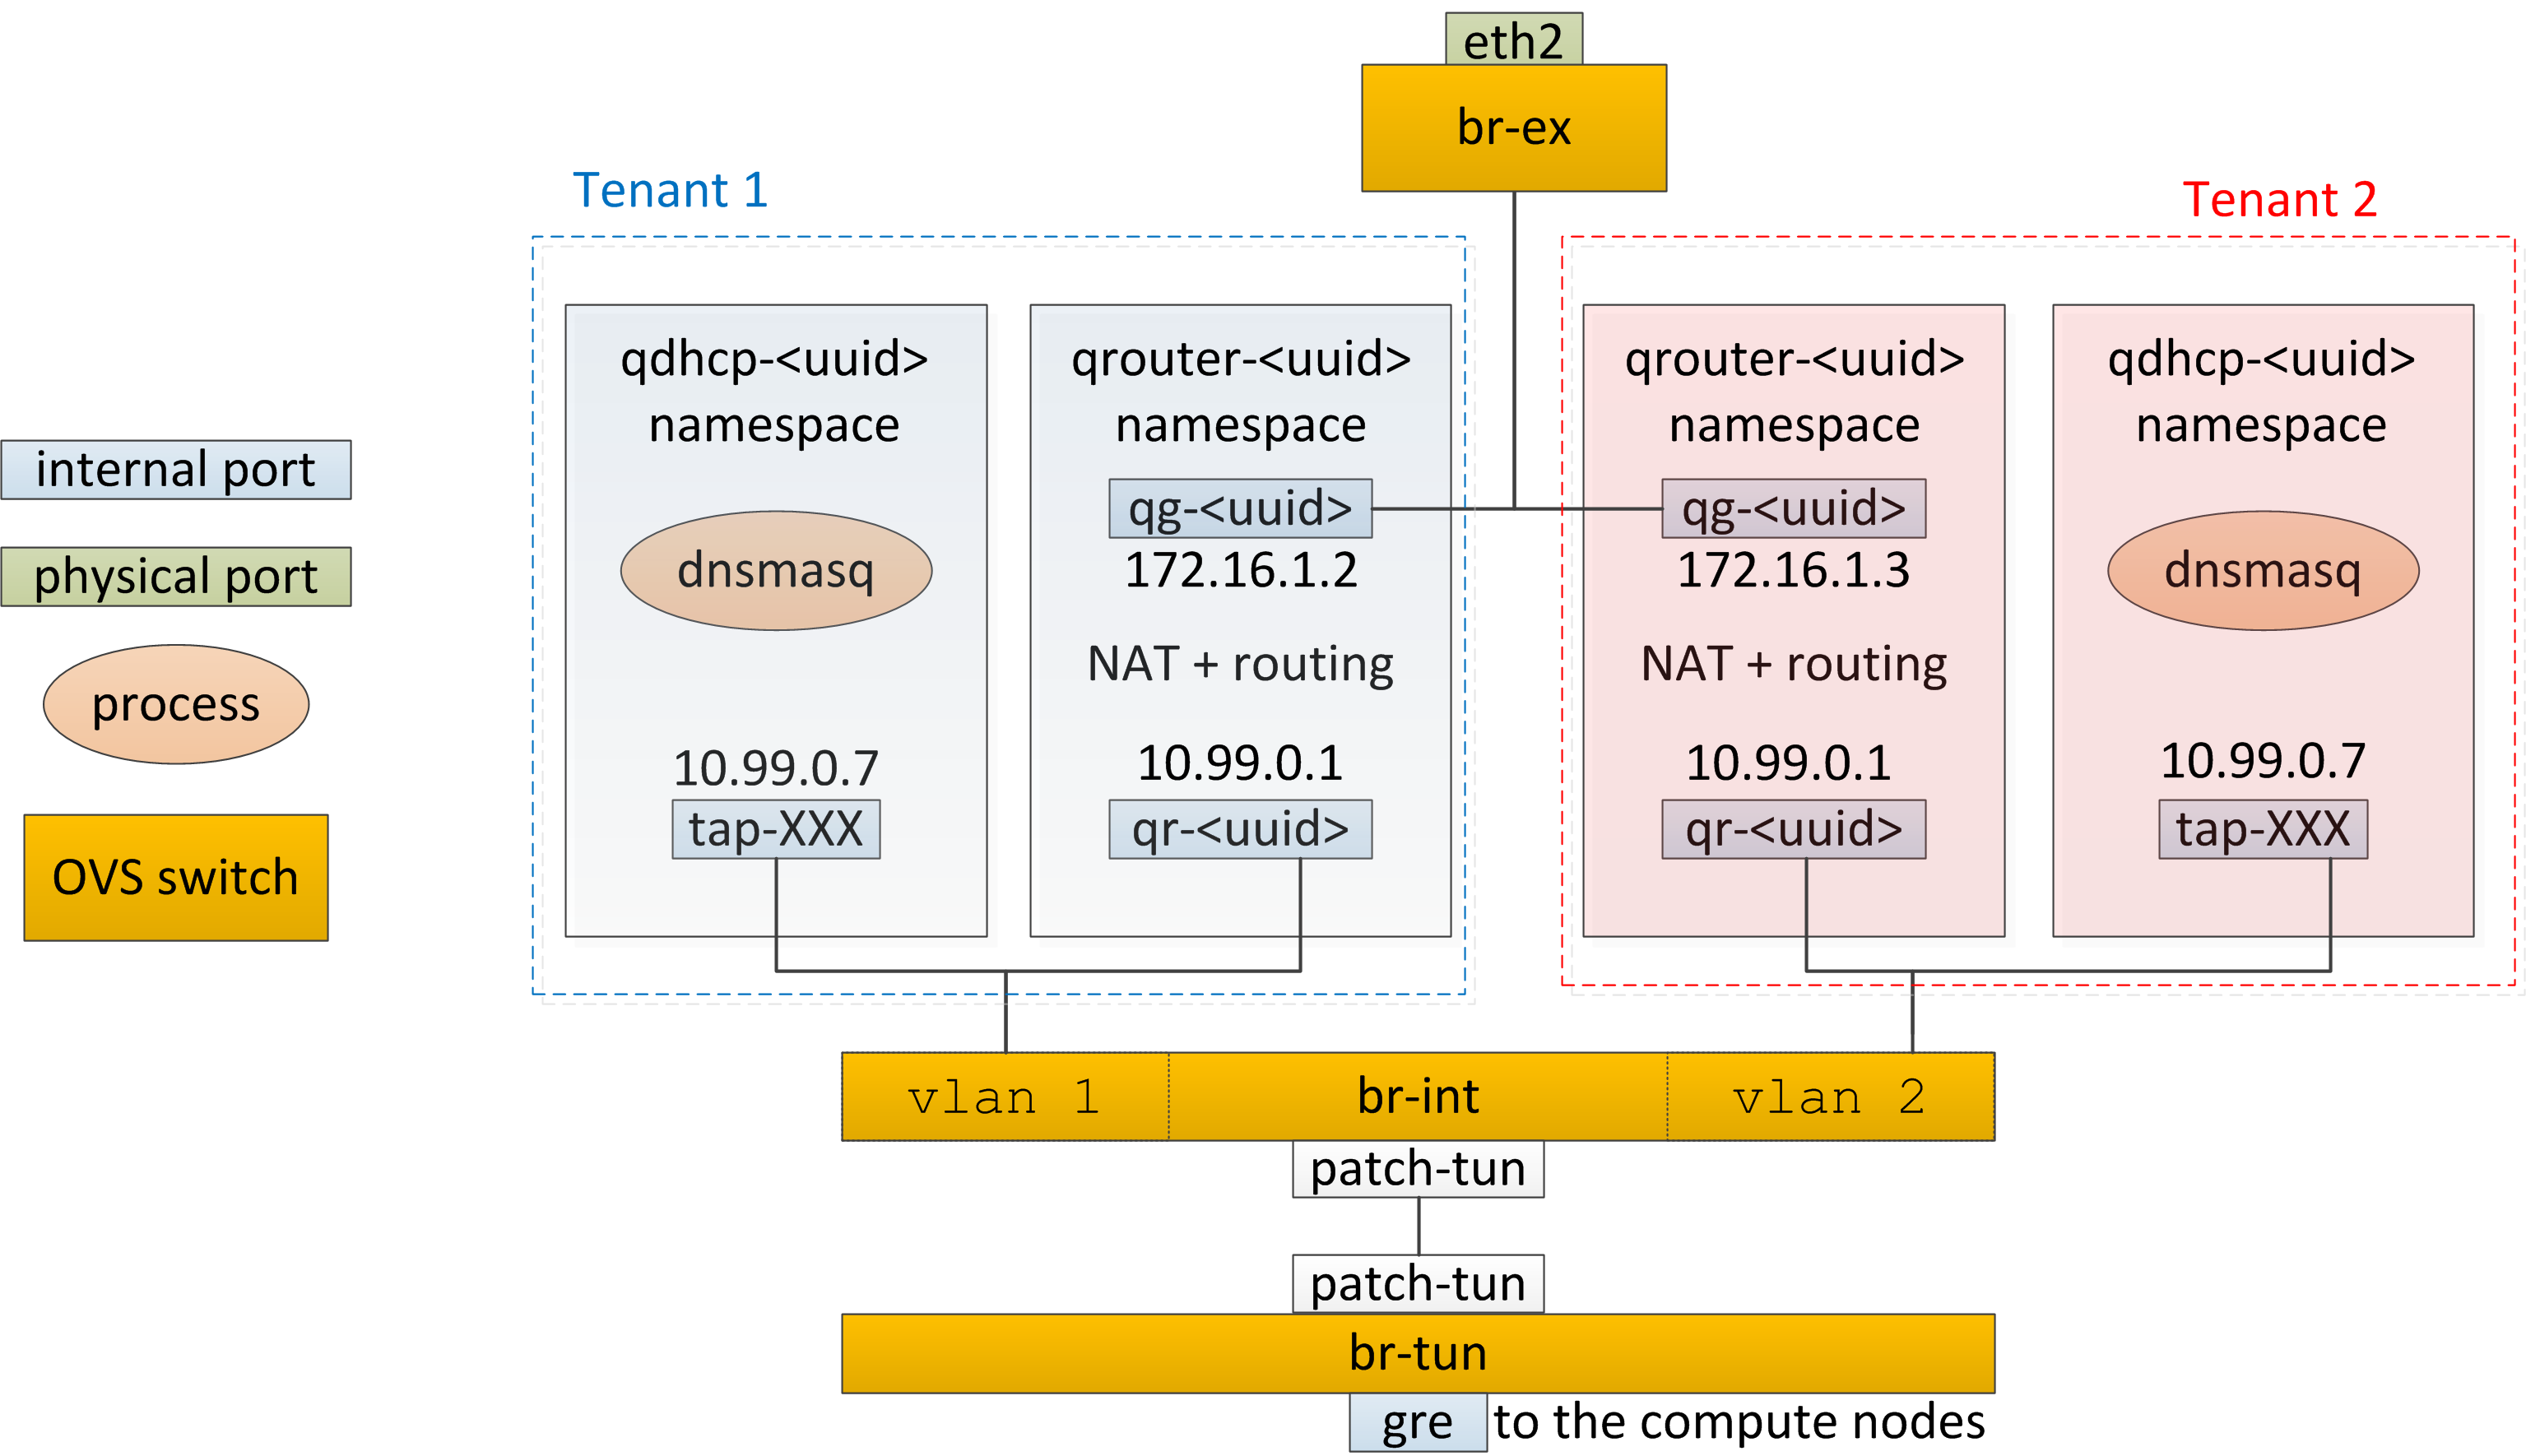
\includegraphics[width=\linewidth]{under-the-hood-neutron-server}
\end{frame}

\begin{frame}
  {Under the hood - compute node}
  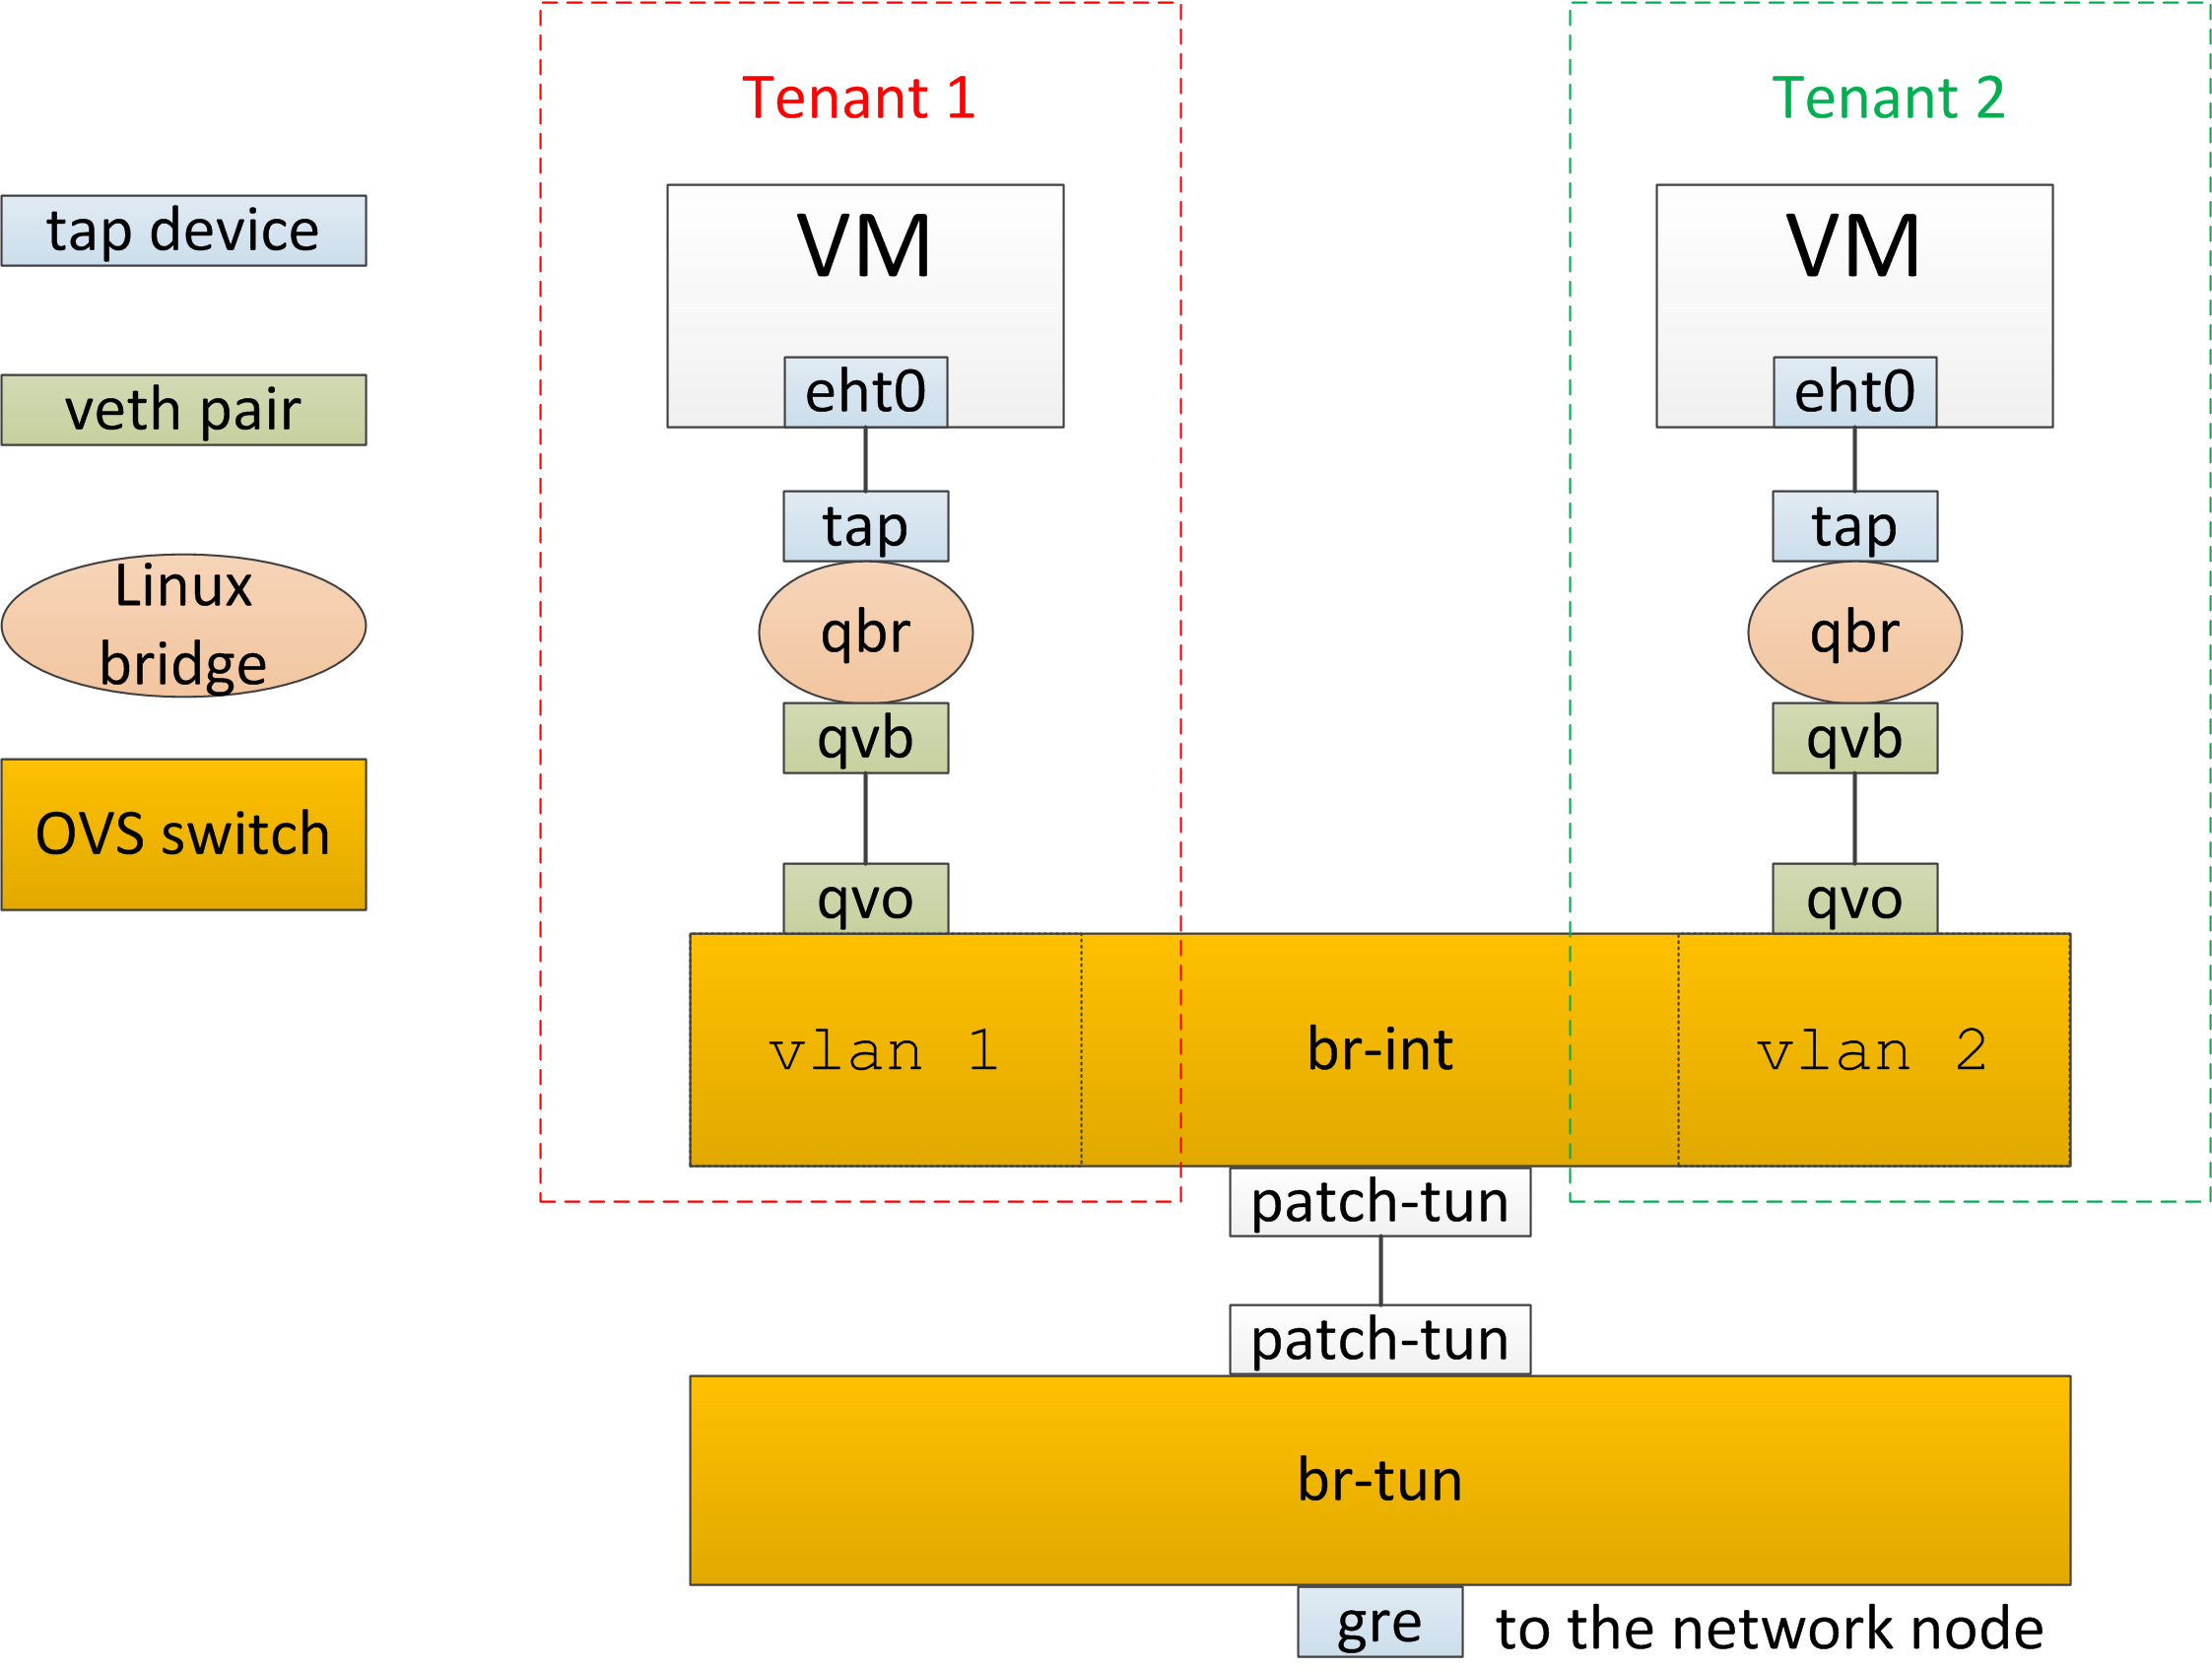
\includegraphics[width=\linewidth]{under-the-hood-compute}
\end{frame}

\begin{frame}
  {easy peasy}
  \begin{figure}[ht]
    \centering
    
\includegraphics[height=20em]{badtime.jpg}
  \end{figure}
\end{frame}

\begin{frame}
  {Metadata proxy}

  \begin{itemize}
  \item usually embededd in the L3 agent

  \item can also be managed by the dhcp agent (useful for \textit{isolated} network)

  \item gets the request from the client, and redirect to the api node

  \item uses IP address 169.254.169.254
  \item requires a client on the VM (cfr \href{https://launchpad.net/cloud-init}{cloud-init})

  \end{itemize}
\end{frame}

\begin{frame}
  {References}
  \begin{itemize}
  \item \href{http://docs.openstack.org/admin-guide-cloud/content/ch_networking.html}{Cloud
      Administrator Guide - Chapter 7 - Networking}
  \item \url{https://wiki.openstack.org/wiki/Neutron}
  \item \href{http://www.confreaks.com/videos/3533-openstacksummitatl2014-inside-the-architecture-of-neutron}{OpenStack
      Summit Atlanta 2014 - Inside the Architecture of Neutron}

  \end{itemize}
\end{frame}

% \begin{frame}
%   {Booting a VM}

%   \begin{itemize}
%   \item instance is created but put in pause
%   \item port is created
%     \begin{itemize}
%     \item dhcp agent is notified
%     \end{itemize}
%   \item network device is created by libvirt
%     \begin{itemize}
%     \item nova waits until the device is wired to the port
%     \end{itemize}
%   \item port is wired
%   \item boot 
%   \end{itemize}
% \end{frame}

\end{document}

